\addchap{Impressum}
%Team Vorstellen
\addsec{Projektteam}
\paragraph{\fenkart}
\begin{minipage}{0.37\textwidth}
	\centering
	\includegraphics[width=0.75\textwidth]{Bilder/Personen/lukas}
	\captionof{figure}{\fenkart \label{fig:lukas_fenkart}}
\end{minipage}
\hfill
\begin{minipage}{0.6\textwidth}
    \fenkart \ widmet sich dem Verständnis der bestehenden Komponenten und dem korrekten Auslesen der Messwerte. Er befasst sich auch mit der Selektion der Hardware und mit dem späteren Zusammenbau der Komponenten.
\end{minipage}%
\vspace{1ex}

\paragraph{\mangeng}
\begin{minipage}{0.37\textwidth}
	\centering
	\includegraphics[width=0.75\textwidth]{Bilder/Personen/luca}
	\captionof{figure}{\mangeng \label{fig:luca_mangeng}}
\end{minipage}
\hfill
\begin{minipage}{0.6\textwidth}
     \mangeng \ ist als Projektleiter zuständig für das Projektmanagement. Dazu unterstützt er den Aufbau und die Auswahl der Hardware.
\end{minipage}%
\vspace{1ex}

\paragraph{\pezze}
\begin{minipage}{0.37\textwidth}
	\centering
	\includegraphics[width=0.75\textwidth]{Bilder/Personen/damiano}
	\captionof{figure}{\pezze \label{fig:damiano_pezze}}
\end{minipage}
\hfill
\begin{minipage}{0.6\textwidth}
    \pezze \ befasst sich in der Software im Frontend. Er designt das Programm und setzt es später im Code um. Er konzeptioniert zudem die grundlegenden \acs{json} Konfigurationsdateien und unterstützt beim Zusammenbau der Hardware. 
\end{minipage}%
\vspace{1ex}

\paragraph{\schneider}
\begin{minipage}{0.37\textwidth}
	\centering
	\includegraphics[width=0.75\textwidth]{Bilder/Personen/martin}
	\captionof{figure}{\schneider \label{fig:martin_schneider}}
\end{minipage}
\hfill
\begin{minipage}{0.6\textwidth}
    \schneider \ beschäftigt sich in der Software im Backend, dabei beschäftigt er sich mit dem \gls{modbus} Protokoll und erarbeitet die Logik für die Auswertung im Programm. Auch im Bereich des Frontends unterstützt er, wenn nötig.
\end{minipage}%
\vspace{1ex}

\addsec{Projektbetreuer}
\paragraph{Prof. DI Klaus Battlogg}
\begin{minipage}{0.37\textwidth}
	\centering
	\includegraphics[width=0.75\textwidth]{Bilder/Personen/battlogg}
	\captionof{figure}{Prof. DI Klaus Battlogg \label{fig:klaus_battlogg}}
\end{minipage}
\hfill
\begin{minipage}{0.6\textwidth}
	Herr Klaus Battlogg ist der Betreuungslehrer des Projektes und unterrichtet Fächer wie BDAS (Big Data - Alternative Systems), BDDA (Big Data - Data Analysis), CCDE (Cloud Computing - Development) und CCIN (Cloud Computing - Infrastructure). Durch sein umfassendes Fachwissen ist er die ideale Wahl als Betreuer für dieses Projekt.
\end{minipage}%
\vspace{1ex}

\paragraph{Ing. Simon Köldorfer, BSc.}
\begin{minipage}{0.37\textwidth}
	\centering
	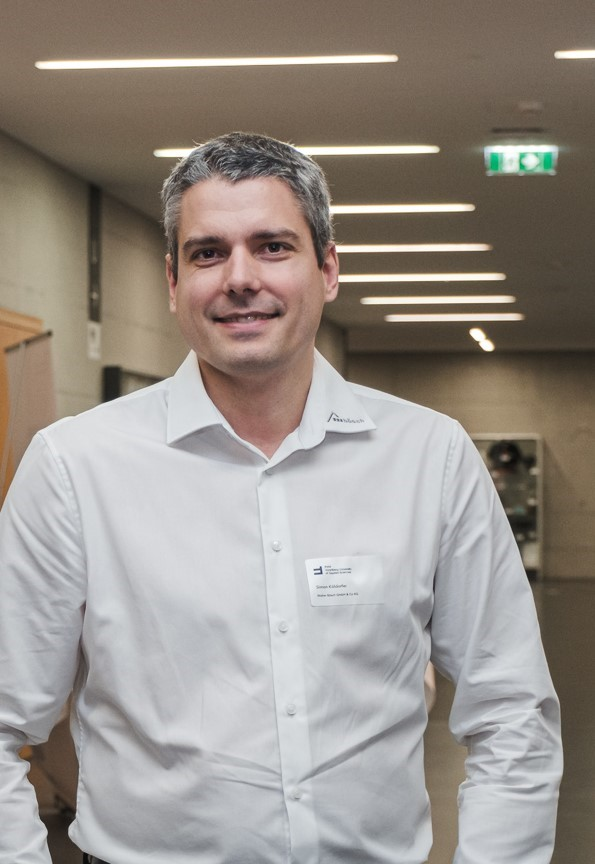
\includegraphics[width=0.75\textwidth]{Bilder/Personen/koeldorfer}
	\captionof{figure}{Ing. Simon Köldorfer, BSc. \label{fig:simon_koeldorfer}}
\end{minipage}
\hfill
\begin{minipage}{0.6\textwidth}
    Herr Simon Köldorfer fungiert als unsere firmeninterne Kontaktperson und steht dem Projekt durch seine Bereitschaft zur Beantwortung von Fragen und Unterstützung zur Verfügung.
\end{minipage}%
\vspace{1ex}